%++++++++++++++++++++++++++++++++++++++++
\documentclass[article, 12pt]{article}
\usepackage{float}
\usepackage{setspace}
\usepackage{tabu} % extra features for tabular environment
\usepackage{amsmath}  % improve math presentation
\usepackage{graphicx} % takes care of graphic including machinery
\usepackage[margin=1in]{geometry} % decreases margins
\usepackage{cite} % takes care of citations
\usepackage[final]{hyperref} % adds hyper links inside the generated pdf file
\usepackage{tikz}
\usepackage{caption} 
\usepackage{fancyhdr}
\usepackage{amssymb} % symbols like /therefore
\usepackage{amsthm} % proofs
\usepackage{enumerate} % lettered lists
\usepackage{mathtools} % macros
\usetikzlibrary{scopes}
% \usepackage{xcolor} \pagecolor[rgb]{0.12549019607,0.1294117647,0.13725490196} \color[rgb]{0.82352941176,0.76862745098,0.62745098039} % dark theme
\theoremstyle{definition}
\newtheorem{example}{Example}
\newtheorem*{remark}{Remark}
\newtheorem{theorem}{Theorem}[subsection]
\newtheorem{definition}{Definition}
\newcommand*{\Definitionautorefname}{Definition}
\newtheorem{corollary}{Corollary}[subsection]
\hypersetup{
	colorlinks=false,      % false: boxed links; true: colored links
	linkcolor=blue,        % color of internal links
	citecolor=blue,        % color of links to bibliography
	filecolor=magenta,     % color of file links
	urlcolor=blue         
}
\usepackage{physics}
\usepackage{siunitx}
\usepackage{tikz,pgfplots}
\usepackage{subcaption} % subfigures
\usepackage[outline]{contour} % glow around text
\usetikzlibrary{calc}
\usetikzlibrary{angles,quotes} % for pic
\usetikzlibrary{arrows.meta}
\tikzset{>=latex} % for LaTeX arrow head
\contourlength{1.2pt}

\colorlet{xcol}{blue!70!black}
\colorlet{vcol}{green!60!black}
\colorlet{myred}{red!70!black}
\colorlet{myblue}{blue!70!black}
\colorlet{mygreen}{green!70!black}
\colorlet{mydarkred}{myred!70!black}
\colorlet{mydarkblue}{myblue!60!black}
\colorlet{mydarkgreen}{mygreen!60!black}
\colorlet{acol}{red!50!blue!80!black!80}
\tikzstyle{CM}=[red!40!black,fill=red!80!black!80]
\tikzstyle{xline}=[xcol,thick,smooth]
\tikzstyle{mass}=[line width=0.6,red!30!black,fill=red!40!black!10,rounded corners=1,
                  top color=red!40!black!20,bottom color=red!40!black!10,shading angle=20]
\tikzstyle{faded mass}=[dashed,line width=0.1,red!30!black!40,fill=red!40!black!10,rounded corners=1,
                        top color=red!40!black!10,bottom color=red!40!black!10,shading angle=20]
\tikzstyle{rope}=[brown!70!black,very thick,line cap=round]
\def\rope#1{ \draw[black,line width=1.4] #1; \draw[rope,line width=1.1] #1; }
\tikzstyle{force}=[->,myred,very thick,line cap=round]
\tikzstyle{velocity}=[->,vcol,very thick,line cap=round]
\tikzstyle{Fproj}=[force,myred!40]
\tikzstyle{myarr}=[-{Latex[length=3,width=2]},thin]
\def\tick#1#2{\draw[thick] (#1)++(#2:0.12) --++ (#2-180:0.24)}
\DeclareMathOperator{\sn}{sn}
\DeclareMathOperator{\cn}{cn}
\DeclareMathOperator{\dn}{dn}
\def\N{80} % number of samples in plots


\usepackage{titling}
\renewcommand\maketitlehooka{\null\mbox{}\vfill}
\renewcommand\maketitlehookd{\vfill\null}
\usepackage{siunitx} % units
\usepackage{verbatim} 
\newcommand{\courseNumber}{MATH 273}
\newcommand{\courseName}{Discrete Mathematics 2}
\newcommand{\professor}{Dr. Petrescu}
\newcommand{\name}{Denny Cao}
\pagestyle{fancy}
\fancyhf{}% clears all header and footer fields
\fancyfoot[C]{--~\thepage~--}
\renewcommand*{\headrulewidth}{0.4pt}
\renewcommand*{\footrulewidth}{0pt}
\lhead{\name}
\chead{\courseNumber: \courseName}
\rhead{\professor}


\fancypagestyle{plain}{%
  \fancyhf{}% clears all header and footer fields
  \fancyfoot[C]{--~\thepage~--}%
  \renewcommand*{\headrulewidth}{0pt}%
  \renewcommand*{\footrulewidth}{0pt}%
}

% Shortcuts
\DeclarePairedDelimiter\ceil{\lceil}{\rceil} % ceil function
\DeclarePairedDelimiter\floor{\lfloor}{\rfloor} % floor function

\DeclarePairedDelimiter\paren{(}{)} % parenthesis

\newcommand{\df}{\displaystyle\frac} % displaystyle fraction
\newcommand{\qeq}{\overset{?}{=}} % questionable equality

\newcommand{\Mod}[1]{\;\mathrm{mod}\; #1} % modulo operator

% Sets
\DeclarePairedDelimiter\set{\{}{\}}
\newcommand{\unite}{\cup}
\newcommand{\inter}{\cap}

\newcommand{\reals}{\mathbb{R}} % real numbers: textbook is Z^+ and 0
\newcommand{\ints}{\mathbb{Z}}
\newcommand{\nats}{\mathbb{N}}
\newcommand{\rats}{\mathbb{Q}}

\newcommand{\degree}{^\circ}

% Div Operator
\makeatletter
\newcommand*{\bdiv}{%
  \nonscript\mskip-\medmuskip\mkern5mu%
  \mathbin{\operator@font div}\penalty900\mkern5mu%
  \nonscript\mskip-\medmuskip
}
\makeatother

\newcommand{\comp}{\circ} % composite

% Counting
\newcommand\perm[2][^n]{\prescript{#1\mkern-2.5mu}{}P_{#2}}
\newcommand\comb[2][^n]{\prescript{#1\mkern-0.5mu}{}C_{#2}}

% Relations
\newcommand{\rel}{\mathrel{R}} % relation

\setlength\parindent{0pt}

% Sign Charts
\newdimen\tcolw \tcolw=2.5em % the column width
\edef\ecatcode{\catcode`&=\the\catcode`&\relax}\catcode`&=4
\def\sgchart#1#2{\vbox{\offinterlineskip\halign{\hfil##\quad&##\hfil\crcr\sgchartA#2,:,%
   \omit\sgchartR&\kern.2pt\sgchartS{.5\tcolw}\relax\sgchartE#1,\relax,%
   \sgchartS{.5\tcolw}\relax\cr
   \noalign{\kern2pt}&\def~{}\kern.5\tcolw\sgchartD#1,\relax,\cr}}}
\def\sgchartA#1:#2,{\cr\ifx,#1,\else $#1$&\sgchartB#2{}\expandafter\sgchartA\fi}
\def\sgchartB#1{\hbox to\tcolw{\hss$#1$\hss}\sgchartC}
\def\sgchartC#1{\ifx,#1,\else
   \strut\vrule\kern-.4pt\hbox to\tcolw{\hss$#1$\hss}\expandafter\sgchartC\fi}
\def\sgchartD#1#2,{\ifx\relax#1\else\hbox to\tcolw{\hss$#1#2$\hss}\expandafter\sgchartD\fi}
\def\sgchartE#1#2,{\ifx\relax#1\else
    \ifx~#1\sgchartS\tcolw\circ \else\sgchartS\tcolw\bullet\fi \expandafter\sgchartE\fi}
\def\sgchartR{\leaders\vrule height2.8pt depth-2.4pt\hfil}
\def\sgchartS#1#2{\hbox to#1{\kern-.2pt\sgchartR \ifx\relax#2\else
   \kern-.7pt$#2$\kern-.7pt\sgchartR\fi\kern-.2pt}}
\ecatcode
%++++++++++++++++++++++++++++++++++++++++
\title{
    \vspace{2in}
    \textmd{\textbf{\courseNumber: \courseName}}
    \normalsize\vspace{0.1in}\\
    \vspace{0.1in}\large{\text{\professor}}
    \vspace{3in}
}

\author{\name}
\date{Final: April 26, 2023}

\begin{document}
    \maketitle
    \thispagestyle{empty}
    \pagebreak
    \tableofcontents
    \pagebreak
    \setcounter{section}{8}
    \section{Relations}
    \subsection{Relations and Their Properties}
    \subsubsection{Introduction}
    \begin{definition}\label{def:cartesian product}
            Let $A$ and $B$ be sets. The \textbf{cartesian product} of $A$ and $B$ is the set
                \[ A \times B = \set*{(a, b) \mid a \in A \land b \in B} \]
        \end{definition}
        \begin{itemize}
            \item $A \times B \neq B \times A$
            \item Every function is a relation, but not every relation is a function. When it is a function, it is one-to-one.
        \end{itemize}
    
    \begin{definition}\label{def:binary relation}
        Let $A$ and $B$ be sets. A \textbf{binary relation from $A$ to $B$} is a subset of $A \times B$.
    \end{definition}
    \begin{itemize}
        \item A binary relation from $A$ to $B$ is a set $R$ of ordered pairs. First element is from $A$, second element is from $B$.
        \item We use notation $a \rel b$ to denote $(a, b) \in R$.
        \item We use notation $a \not \rel b$ to denote $(a, b) \not \in R$.
        \item When $(a,b)$ belongs to $R$, $a$ is \textbf{related to} $b$.
        \item Recall there are $2^{|S|}$ subsets of $S$. These are the amount of relations from $A$ to $B$. Remember that this includes $\emptyset$.

    \end{itemize}
    \begin{example}
        Let $A = \set*{0,1,2}$ and $B=\set*{a,b}$. Then $\set*{(0,a),(0,b),(1,a),(2,b)}$ is a relation from $A$ to $B$. This means, for instance, that $0 \mathrel{R} a$, but that $1 \not \mathrel{R} b$. Relations can be represented graphically:
        \begin{figure}[H]\label{fig:relation}
            \centering
            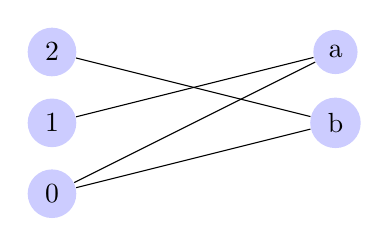
\begin{tikzpicture}
                [scale=.9,auto=center,every node/.style={circle,fill=blue!20}]
                \node (a0) at (0,0) {0};
                \node (a1) at (0,1) {1};  
                \node (a2) at (0,2) {2}; 

                \node (aA) at (4,2) {a};  
                \node (aB) at (4,1) {b};  

                
                \draw (a0) -- (aA);
                \draw (a0) -- (aB);
                \draw (a1) -- (aA);
                \draw (a2) -- (aB);
            \end{tikzpicture}
            \caption{A relation from $A$ to $B$}
        \end{figure}
        Another way is to use a table:
        \begin{figure}[H]\label{fig:relation table}

            \centering
            \begin{tabular}{c|c c} 
                $\rel$ & $a$ & $b$ \\
                \hline
                0 & 1 & 1 \\
                1 & 1 & 0 \\
                2 & 0 & 1 \\
            \end{tabular}
            \caption{A relation from $A$ to $B$}
        \end{figure}
    \end{example}
    \setcounter{subsubsection}{2}
    \subsubsection{Relations on a Set}
    \begin{definition}
        A \textbf{relation on a set} $A$ is a relation from $A$ to $A$
    \end{definition}
    \begin{example}
        Let $A$ be the set $\set*{1,2,3,4}$. Which ordered pairs are in the relation $R = \set*{(a,b) \mid a \bdiv b}$?
        \begin{figure}[H]
            \centering
            \begin{tabular}{c|c c c c}
                $R$ & 1 & 2 & 3 & 4 \\
                \hline
                1 & 1 & 1 & 1 & 1 \\
                2 & 0 & 1 & 0 & 1 \\
                3 & 0 & 0 & 1 & 0 \\
                4 & 0 & 0 & 0 & 1 \\
            \end{tabular}
            \label{fig:example 1.1.2}
        \end{figure}
        \begin{itemize}
            \item Note that this can be a matrix!
        \end{itemize}
    \end{example}
    \subsubsection{Properties of Relations}
    \begin{definition}\label{def:reflexive}
        A relation $R$ on a set $A$ is called \textbf{reflexive} if
            \[ \forall a \in A((a,a) \in R) \]
    \end{definition}
    \begin{itemize}
        \item If the relation is reflexive, then \textbf{the main diagonal of the matrix is full}
    \end{itemize}
    \begin{definition}\label{def:symmetric and antisymmetric}
        A relation $R$ on a set $A$ is called \textbf{symmetric} if:
            \[ \forall a \forall b \in A((a,b) \in R \rightarrow (b,a) \in R) \]
        A relation $R$ on a set $A$ is called \textbf{antisymmetric} if:
            \[ \forall a \forall b \in A((a,b) \in R \land (b,a) \in R \rightarrow (a=b)) \]
    \end{definition}
    \begin{itemize}
        \item If the relation is symmetric, then \textbf{the matrix is symmetric}. This means that $A = A^T$, and can be seen if the upper and lower triangles are the same.
        \item If the matrix is antisymmetric, then it does not necessarily mean that the \textbf{relation} is antisymmetric.
    \end{itemize} 
    \begin{definition}
    \label{def:transitive}
        A relation $R$ on a set $A$ is called \textbf{transitive} if:
            \[ \forall a \forall b \forall c \in A((a,b) \in R \land (b,c) \in R \implies (a,c) \in R) \]
    \end{definition}
    \begin{figure}[H]
        \centering
        \begin{subfigure}{.25\textwidth}
            \centering
            \[ \begin{bmatrix}
               1 & & & & & & \\
               & 1 & & & & & \\
               & & 1 & & & & \\
               & & & 1 & & & \\
               & & & & 1 & & \\
               & & & & & 1 & \\
               & & & & & & 1 \\
               \end{bmatrix} \] 
        \caption{Reflexive}
        \end{subfigure}
    \newcommand\tikznode[2]{\tikz[remember picture,baseline=(#1.base)]{\node(#1)[inner sep=0pt]{#2};}}
    \begin{subfigure}{.25\textwidth}
        \centering
        \[ \begin{bmatrix}
            \tikznode{d1}{} & & & & \tikznode{a}{1} &   \\
            & & & & & & &  \\
            & & & & & & \tikznode{c}{0} &   \\
            & & & & & & &  \\
            \tikznode{b}{1} & & & & & &   \\
            & & & & & & & \\
            & & \tikznode{d}{0} & & & & &  \tikznode{d2}{} \\
        \end{bmatrix} \]
        \tikz[overlay,remember picture]{\draw[-, myred](a)--(b); \draw[-, myred](c)--(d); \draw[-](d1)--(d2);}
        \caption{Symmetric}
    \end{subfigure}
    \begin{subfigure}{.25\textwidth}
        \centering
        \[ \begin{bmatrix}
            \tikznode{d1}{} & & & & \tikznode{a}{1} &   \\
             & & & & &\tikznode{e}{1} &   \\
            & & & & & & \tikznode{c}{0} &   \\
            & & & & & & &  \\
            \tikznode{b}{0} & & & & & &   \\
            & \tikznode{f}{0} & & & & &  \\
            & & \tikznode{d}{1} & & & & &  \tikznode{d2}{} \\
        \end{bmatrix} \]
        \tikz[overlay,remember picture]{\draw[-, myred](a)--(b); \draw[-, myred](c)--(d); \draw[-, myred](e)--(f); \draw[-](d1)--(d2);}
        \caption{Antisymmetric}
    \end{subfigure}
    \end{figure}
    \subsubsection{Combining Relations}
    Similar to composing functions. We can combine relations in any way two sets can be combined. You can do everything you can do with sets. 
    \begin{definition}
        Let $R$ be a relation from a set $A$ to a set $B$ and $S$ a relation from $B$ to a set $C$. The \textbf{composite} of $R$ and $S$ is the relation consisting of ordered pairs $(a,c)$, where $a \in A, c \in C$, and for which $\exists b \in B \mid (a,b) \in R \land (b,c) \in S$. We denote the composite of $R$ and $S$ by $S \comp R$.
    \end{definition}
    \begin{itemize}
        \item If there is an $A$ in $R$ that maps to $B$, and for $S$ there is a $B$ that maps to a $C$, then the composite $S \comp R$ will map $A$ to $C$.
        \item If $B$ maps to multiple $C$'s?, then the composite will map $A$ to multiple $C$'s.
    \end{itemize}
    \begin{definition}\label{def:reflexive powers}
        Let $R$ be a relation on the set $A$. The powers $R^n$, $n=1,2,3,\dots$ are defined recursively by:
            \[ R^1 = R \quad \text{and} \quad R^{n+1} = R \comp R^n \]
    \end{definition}
    \begin{definition}\label{def:transitive theorem}
        The relation $R$ on a set $A$ is \textbf{transitive} if and only if: 
        \[ \forall n \geq 1, R^n \subseteq R \]
    \end{definition}
    \subsection{$n$-ary Relations and Their Applications}
    \setcounter{definition}{0}
    \setcounter{example}{0}
    \subsubsection{$n$-ary Relations}
    \begin{definition}\label{def:nary}
        Let $A_1, A_2, \dots, A_n$ be sets. An \textbf{$n$-ary relation} is a subset of $A_1 \times A_2 \times \dots \times A_n$. The sets $A_1, A_2, \dots, A_n$ are called the \textbf{domains} of the relation, and $n$ is called its degree.
    \end{definition}
    \begin{example}
        Let $R$ be the relation consisting of 4-tuples $(A, N, S, D, T)$ representing airplane flights, where $A$ is the airline, $N$ is the flight number, $S$ is the starting point, $D$ is the destination, and $T$ is the departure time. The degree of this relation is 5, and its domains are the set of airlines, the set of flight numbers, the set of cities, the set of cities (again), and the set of times. 
    \end{example}
    \subsubsection{Databases and Relations}
    
    \subsubsection{Matrix Representation}
    Suppose $A = \set*{1,2,3}$ and $B = \set*{1,2}$. Let $\mathrel{R}$ be the relation from $A$ to $B$ containing $(a,b)$ if $a \in A, b \in B$, and $a > b$. The matrix representation of $\mathrel{R}$ if $a_1 = 1, a_2 = 2$, and $a_3 = 3$, and $b_1 = 1$ and $b_2 = 2$ is:
    \begin{figure}[H]
        \[ \begin{bmatrix}
            0 & 0 \\
            1 & 0 \\
            1 & 1
        \end{bmatrix} \] 
    \end{figure}
    \begin{itemize}
        \item The number of rows is the size of $A$. The number of columns is the size of $B$. 
        \item This is the set: $A \mathrel{R} B = \set*{(2,1), (3,1), (3,2)}$.
    \end{itemize}
    Let $a_{ij}$ represent an element in a matrix in the $i$th row and the $j$th column:
    \begin{figure}[H]
        \[ A = \begin{bmatrix}
            a_{11} & a_{12} & a_{13} \\
            a_{21} & a_{22} & a_{23} \\
            a_{31} & a_{32} & a_{33}
        \end{bmatrix} \]
    \end{figure}
    \begin{itemize}
        \item A relation is \textbf{reflexive} if the main diagonal is all 1: $a_{11} = a_{22} = a_{33} = a_{ii}$
        \item A relation is \textbf{symmetric} if $a_{ij} = a_{ji}$. This implies that $A^T = A$.
        \item We can figure out if a relation is \textbf{antisymmetric} by using \autoref{def:transitive theorem}. Suppose the relations $R_1$ and $R_2$ are represented by:
        \[ M_{R_1} = \begin{bmatrix}
            1 & 0 & 1 \\
            1 & 1 & 0 \\
            0 & 0 & 0
        \end{bmatrix} \text{ and } M_{R_2} = \begin{bmatrix}
            0 & 1 & 0 \\
            0 & 0 & 1 \\
            1 & 0 & 1
        \end{bmatrix}\]
        The composition of these two matrices is the boolean product of them, from \autoref{def:reflexive powers}. Let $M_{R_1} = A$ and $M_{R_2} = B$. Then the composite of $R_1$ and $R_2$ is:
        \[ A \odot B = \begin{bmatrix}
            A_{\text{row 1}} \cdot B_{\text{col 1}} & A_{\text{row 1}} \cdot B_{\text{col 2}} & A_{\text{row 1}} \cdot B_{\text{col 3}} \\
            A_{\text{row 2}} \cdot B_{\text{col 1}} & A_{\text{row 2}} \cdot B_{\text{col 2}} & A_{\text{row 2}} \cdot B_{\text{col 3}} \\
            A_{\text{row 3}} \cdot B_{\text{col 1}} & A_{\text{row 3}} \cdot B_{\text{col 2}} & A_{\text{row 3}} \cdot B_{\text{col 3}}
        \end{bmatrix} = \begin{bmatrix}
            1 & 1 & 1 \\
            0 & 1 & 1 \\
            0 & 0 & 0
        \end{bmatrix} \] 
        If $R_1$ is contained in $R_2$, then $R_1$ is antisymmetric.
    \end{itemize}
    % Read this part and understand. Confused on what in the fuck is happening here

    We can represent relations as directed graphs. The following is a directed graph with verticies $a, b, c,$ and $d$, and edges $(a,b), (a,d), (b,b), (b,d), (c,a), (c,b),$ and $(d,b)$:
    \begin{figure}[H]
        \centering
        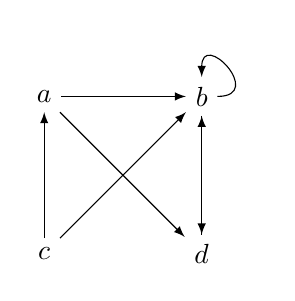
\begin{tikzpicture}
            \node (a) at (0,0) {$a$};
            \node (b) at (2,0) {$b$};
            \node (c) at (0,-2) {$c$};
            \node (d) at (2,-2) {$d$};
            \draw[->] (a) to (b);
            \draw[->] (a) to (d);
            \draw[->] (b) to [out=0,in=-270,looseness=5] (b);
            \draw[->] (b) to (d);
            \draw[->] (c) to (a);
            \draw[->] (c) to (b);
            \draw[->] (d) to (b);
        \end{tikzpicture}
    \end{figure}
    % Figure out how to make this look better. For the bidirectional edges, I want to make it curved. Arrows in the middle. Also, for the loop, how to make it more circular.
    \begin{itemize}
        \item \textbf{Reflexive} if there is a loop on every vertex. 
        \item \textbf{Symmetric} if every edge is bidirectional.
    \end{itemize}
        
\end{document}
 